%
%Free under Creative Commons Attribution-NonCommercial 4.0 International (CC BY-NC 4.0)
%

\documentclass[12pt]{article}
\usepackage{fancyhdr}
\usepackage{color}
\usepackage{multicol}
\usepackage{enumitem}
\usepackage{graphicx}
\usepackage{sectsty}
\usepackage{amsmath}
\usepackage{amssymb}
\usepackage{hyperref}
\usepackage{array}
\usepackage{alltt}
\newcommand{\sectionbreak}{\clearpage}
\usepackage[first=-10, last=30]{lcg}

\usepackage{tikz}
	\usetikzlibrary{arrows,shapes,trees}

\usepackage{tkz-euclide}
\usetkzobj{all}

\allsectionsfont{\centering}

\usepackage{draftwatermark}
	\SetWatermarkText{wolf-math.com}
	\SetWatermarkScale{5}
	\SetWatermarkAngle{90}
	\SetWatermarkLightness{1}

\usepackage[margin=1in, headsep=0pt]{geometry}
\setlength{\parindent}{0cm}
%\pagestyle{empty}

\let\stdsection\section
\renewcommand\section{\newpage\stdsection}

\begin{document}
\newcommand{\random}{\rand\arabic{rand}}

\tableofcontents

\section{Function Notation \& Inverse Functions}


Mr. Wolf \\ wolf-math.com

\subsection{Goals}

\textbf{SWBAT} use function notation to write functions\\

\textbf{SWBAT} perform operations on functions using function notation\\

\textbf{SWBAT} perform compositions of functions\\

\textbf{SWBAT} identify inverse functions by composing one into another\\

\textbf{SWBAT} create inverse functions


\subsection{Standards}

\textbf{Interpreting Functions \hfill F-IF}\\

1. Understand that a function from one set (called the domain) to
another set (called the range) assigns to each element of the domain
exactly one element of the range. If f is a function and x is an element
of its domain, then f(x) denotes the output of f corresponding to the
input x. The graph of f is the graph of the equation y = f(x).\\

2. Use function notation, evaluate functions for inputs in their domains,
and interpret statements that use function notation in terms of a
context.\\

\textbf{Building Functions \hfill F-BF}

Build new functions from existing functions\\

3. Identify the effect on the graph of replacing $f(x)$ by $f(x) + k$, $k f(x)$,
$f(kx)$, and $f(x + k)$ for specific values of $k$ (both positive and negative);
find the value of $k$ given the graphs. Experiment with cases and
illustrate an explanation of the effects on the graph using technology.
Include recognizing even and odd functions from their graphs and
algebraic expressions for them.\\

4. Find inverse functions.\\

a. Solve an equation of the form $f(x) = c$ for a simple function $f$
that has an inverse and write an expression for the inverse. For
example, $f(x) =2 x^3$ for $x > 0$ or $f(x) = (x+1)/(x–1)$ for $x ≠ 1$.\\

b. (+) Verify by composition that one function is the inverse of
another.\\

c. (+) Read values of an inverse function from a graph or a table,
given that the function has an inverse.\\

d. (+) Produce an invertible function from a non-invertible function
by restricting the domain.\\



\subsection{Before \& After}

\textbf{Before} we learned about exponential functions and their applications.\\

\textbf{Now} we are learning about function notation so that we can learn about inverse functions, specifically the inverses of exponential functions (i.e. logarithms).\\

\textbf{After} we will learn about exponential functions, and logarithms, and how logarithms are the inverse functions of exponential functions. 



\section{What is a Function?}

A function is a machine that turns one thing into another. \\

A toaster is a ``function'' that turns bread into toast.\\

A mathematical function is a rule that changes some number or expression into a different number or expression.\\

The input of a function is called the \textbf{DOMAIN}, and the output is called the \textbf{RANGE}.\\

Functions are written with ordered pairs. 

\section{Using Function Notation}

Another perk of using function notation is that you can plug things into the function really easily. If we want to find out when $x=3$ we will write $f(3)$\\

$$\mathbf{f(x)=3x-1}$$

$f(1)=3(1)-1$\\

$f(2)=3(2)-1$\\

$f(3)=3(3)-1$\\

\textbf{You can also plug in other variables. To plug these}\\

\begin{enumerate}
\item Put a set of parenthesis wherever $x$ was\\

\item Then plug your variable/expression into the parenthesis\\

\item Simplify\\
\end{enumerate}


$f(c)=$\\

$f(5r)=$\\

Plug in expressions\\

$f(x+1)=$\\

$f(y^2)=$\\

\hrulefill

\textbf{You Try:}

$$\mathbf{f(x)=x^2-2x-1}$$

\begin{enumerate}

	\item $f(1)=$
	
	\item $f(-1)=$
	
	\item $f(7)=$
	
	\item $f(0)=$
	
\end{enumerate}



\section{Function Notation \& Operations}

\textbf{Function notation} is a common way to write equations. Function notation is written $f(x)$ and read "f of x." When we are dealing with functions it is enough to say $y=f(x)$. $y$ and $f(x)$ are pretty much interchangeable, but there are few things that function notation allows us to do that a regular $y$ doesn't.\\

$$f(x)=2x  \text{ and } g(x)=x+5$$

\vspace{12pt}

\begin{center}
\def\arraystretch{2}%  1 is the default, change whatever you need
\begin{tabular}{l|c|c}

\textbf{Operation} 		& \textbf{Definition} 				& \textbf{Example} \\ \hline
Addition 		& $[f+g](x) = f(x)+g(x)$	& $2x + (x+5)$ \\ \hline
Subtraction 	& $[f-g](x) = f(x)-g(x)$	& $2x - (x+5)$ \\ \hline
Multiplication 	& $[f \cdot g](x) = f(x) \cdot g(x)$ 	& $2x \cdot (x+5)$ \\ \hline
Division 		& $[f \div g](x) = \frac{f(x)}{g(x)}$ 	& $\frac{2x}{x+5}$ \\ 

\end{tabular}
\end{center}

\hspace{12pt}



\hrulefill

\textbf{Example:}\\ $f(x)=3x+4$ \hspace{.5in} and \hspace{.5in} $g(x)=5x-8$ 

\begin{enumerate}
	\item $[f+g](x)=$\\
	
	\item $[f-g](x)=$\\
	
	\item $[g-f](x)=$\\
	
	\item $[f \cdot g](x)=$\\
	
	\item $[f\div g](x)=$\\
\end{enumerate}

\pagebreak

\textbf{You Try} Perform the indicated operations on the two functions.\\

$$h(x)=x-8$$

$$k(x)=5x$$\\

\begin{enumerate}
	\item $[h+k](x)=$\\
	
	\item $[h-k](x)=$\\
	
	\item $[k-h](x)=$\\
	
	\item $[h \cdot k](x)=$\\
	
	\item $\left[\frac{h}{k}\right](x)=$\\
\end{enumerate}

\hrulefill

\textbf{You Try:} Perform the operations on functions.\\

$$p(x)=x+10$$

$$q(x)=2x-10$$

\begin{enumerate}
	\item $[p+q](x)=$\\
	
	\item $[p \cdot q](x)=$\\
	
	\item $\left[\frac{p}{q}\right] (x)=$\\
	
	\item $[q-p](x)=$\\
	
	\item $[p-q](x)=$\\
\end{enumerate}





\section{Composition of Functions}

Composition of functions means that we can put a function inside a function. There are two equivalent ways to write composition of functions.\\

$$f(x)=2x \hspace{.25in} g(x)=x^3$$

$$[f \circ g](x)= f[g(x)]=f(x^3)$$\\



\textbf{3-step process}  \\

Step 1) Write out $f(x)$ with parenthesis around where the $x$ would be $$2(\hspace{.5cm})$$\\

Step 2) Fill in the blank spots with $g(x)$ $$2(x^3)$$\\

Step 3) Combine like-terms and simplify $$2x^3$$\\

\hrulefill

These are not commutative. Therefore it's going to be different if we write $$[g \circ f](x)$$

Step 1) Write $g(x)$ with parenthesis around where the $x$ would be $$(\hspace{.5cm})^3$$

Step 2) Fill in the blank spots with $f(x)$ $$(2x)^3$$

Step 3) Combine like-terms and simplify $$2^3x^3=8x^3$$



\textbf{Example 2} Compose the functions. $h(x)=x+2$ and $k(x)=2x^2$\\

$$[h \circ k](x)=$$

\vspace{1in}

$$[k \circ h](x)=$$

\vspace{1in}

\hrulefill

\textbf{You Try:} Compose the Functions. $p(x)=5x+5$ and $q(x)=x-10$\\

$$[p \circ q](x)=$$

\vspace{1in}

$$[q \circ p](x)=$$

\pagebreak

\textbf{Directions:} Compose the functions as indicated.

\begin{large}
$$ f(x)=x+3$$

$$g(x)=x^2$$

$$h(x)=5x$$\\
\end{large}

\begin{enumerate}
\begin{multicols}{2}

\item $[f \circ g](x)=$\\

	\vspace{1in}

\item $[g \circ h](x)=$\\

	\vspace{1in}


\item $[f \circ h](x)=$\\

	\vspace{1in}

\item $[g \circ f](x)=$\\

	\vspace{1in}

\item $[h \circ g](x)=$\\

	\vspace{1in}

\item $[h \circ f](x)=$\\

	\vspace{1in}

\end{multicols}
\end{enumerate}






\section{Function Notation Review }

\hfill NAME:\underline{\hspace{3in}}

Review day for function notation. This worksheet is due at the end of class.\\

\subsection{Function Notation \& Operations}



\textbf{Directions:} Complete the following operations on the above listed functions.\\ Use $f(x)=3x-10$ \hspace{.3in} and \hspace{.3in} $h(x)=3x$\\

\begin{enumerate}
\begin{multicols}{2}

	\item $[f+h](x)=$\\
	
	\item $[f-h](x)=$\\
	
	\item $[h-f](x)=$\\
	
	\item $[f \cdot h](x)=$\\
	
	
\end{multicols}
\end{enumerate}

\hrulefill

\subsection{Using Function Notation}

\textbf{Directions:} Plug the numbers or expressions into function notation\\ Use $f(x)=3x-10$ \hspace{.3in} and \hspace{.3in} $h(x)=3x$

\begin{enumerate}[resume]

	\item $f(3)=$\\
	
	\item $f(16)=$\\
	
	\item $h(-12)=$\\
	
	\item $h(0)=$\\
	
	\item $f(2y)=$\\
	
	\item $h(2y)=$\\
	
	\item $f(p+14)=$\\
	
	\item $h(2b^2)=$\\
\end{enumerate}



\subsection{Composition of Functions}

\textbf{Directions:} Use the following functions and compose them as each question indicates.

 $$p(x)=5x-10$$ $$r(x)=9x$$  $$t(x)=x^2$$
 
\begin{enumerate}[resume]

	\item $[p \circ r](x)=$\\
	
		\vspace{1cm}
	
	\item $[p \circ t](x)=$\\
				\vspace{1cm}
	
	\item $[r \circ p](x)=$\\

		\vspace{1cm}
	
	\item $[r \circ t](x)=$\\

		\vspace{1cm}
	
	\item $[t \circ p](x)=$\\

		\vspace{1cm}
	
	\item $ [p \circ p](x)=$\\

\end{enumerate}

Accelerated Objective: A new car dealer is discounting all new cars by 12\%. At the same time, the manufacturer is offering a \$1500 rebate on all new cars. Mr. Slaughter is buying a car that is priced \$24,500. Will the final price be lower if the discount is applied before the rebate or if the rebate is applied before the discount?\\

Let x represent the original price of a new car, $d(x)$ represent the price of a car after the discount, and $r(x)$ represent the price of the car after the rebate.

\section*{Making Connections}

\newcommand{\negspace}{\vspace{-1.5\baselineskip}}

\begin{center}
\bgroup
\def\arraystretch{1.5}
\begin{tabular}{l | p{2.0in}}
Math & Python \\ \hline

$ f(x) = x + 10 $ 
& 
\negspace
\begin{verbatim}
>>> def f(x):
       return x + 10
\end{verbatim}\\

$ g(x) = x^{2} $ &
\negspace
\begin{verbatim}
>>> def g(x):
      return x**2
\end{verbatim}\\ \hline

$ f(7) = 7 + 10 = 17 $ &
\negspace
\begin{verbatim}
>>> f(7)
17
\end{verbatim}\\

$ g(7) = 7^{2} = 49 $ &
\negspace
\begin{verbatim}
>>> g(7)
49
\end{verbatim}\\ \hline

$ f \circ g(7) = f(g(7))$ &
\negspace
\begin{verbatim}
>>> f(g(7))
\end{verbatim}\\

$= f(7^{2}) = f(49) = 59 $ &
\negspace
\begin{verbatim}
>>> f(g(7))
59
\end{verbatim}

\end{tabular}
\egroup
\end{center}

\section{Domain \& Range}

\textbf{Domain:} $x$ values.\\

\textbf{Range:} $y$ values.\\

\hfill simple!\\

\hrulefill

\subsection{Domain and Range from a Graph}

\textbf{Example 1:} Use the graph to determine the \textit{domain} and \textit{range}.

\begin{center}
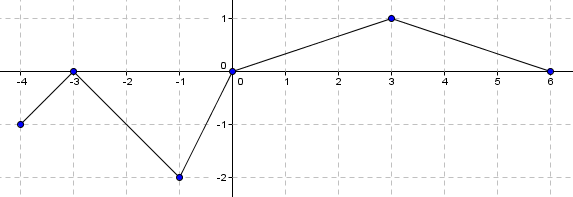
\includegraphics[scale=.5]{domain.png}
\end{center}

\bgroup
\def\arraystretch{1.5}

\begin{center}


\begin{tabular}{ l | c | c | c  }

 & Which values? & Where does the graph go & Answer\\ \hline

\textbf{Domain} & $x$ --values & from -4 to +6 & Domain: [-4,6] \\ \hline

\textbf{Range:}  & $y$--values & from -2 to 1 & Range: [-2,1] \\ \hline

\end{tabular}
\end{center}


\vspace{1cm}

\textbf{Example 2:} Find the domain and range of the graph. $f(x)=x^{2}-2$\\

The hard part of this one is thinking about the \textit{end behavior} of the graph.

\begin{center}
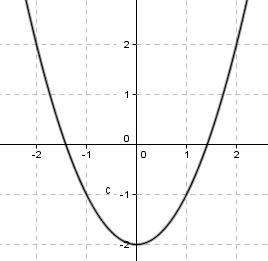
\includegraphics[scale=.5]{domain2.png}\\
\end{center}

\textbf{Domain:}

\vspace{1cm}

\textbf{Range:}\\




\textbf{You Try:} Find the domain and range of the graph.\\

\begin{center}
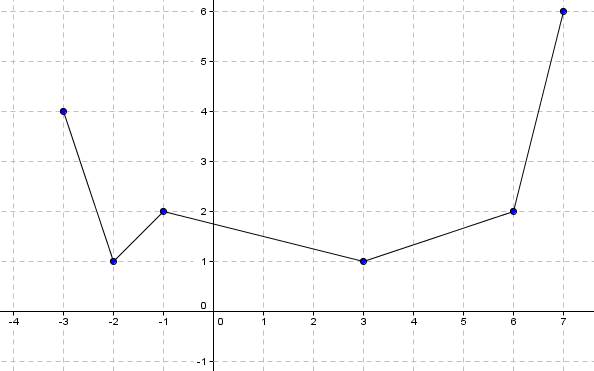
\includegraphics[scale=.5]{domain4.png}\\
\end{center}

\textbf{Domain:}

\vspace{1cm}

\textbf{Range:}\\

\hrulefill

\textbf{You Try:} Find the domain and range of the graph.\\

\begin{center}
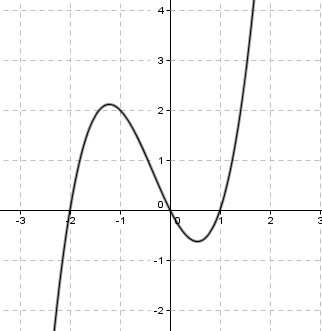
\includegraphics[scale=.5]{domain3.png}\\
\end{center}

\textbf{Domain:}

\vspace{1cm}

\textbf{Range:}\\

\hrulefill

More Practice\\

\url{https://www.khanacademy.org/math/algebra2/functions_and_graphs/domain_range/e/range_of_a_function}

\clearpage



\subsection{Domain and Range from Number Sets}

If we just have a set of numbers we can still determine the \textit{domain} and \textit{range}. \\

Example 1) Determine the domain and range of the data set.\\

$$(-3,18),(7,3),(8,10),(17,-1)$$\\

\begin{multicols}{2}
\begin{center}
	\begin{tabular}{c | c}
	
		smallest $x$ & -3 \\
	
		biggest $x$ & 17\\
	
	\end{tabular}
\end{center}

\begin{center}
	\begin{tabular}{c | c}
	
		smallest $y$ & -1 \\
		
		biggest $y$ & 18\\
	
	\end{tabular}
\end{center}

\end{multicols}

\vspace{1cm}

So the \textbf{domain} is $[-3,17]$\\

and the \textbf{range} is $[-1,18]$\\

\hrulefill

\textbf{You Try:} Find the domain and range of the data set.\\

$$(-2,9),(4,2),(3,3),(10,-3),(-4,11)$$\\

\begin{multicols}{2}
\begin{center}
	\begin{tabular}{c | c}
	
		smallest $x$ &  \\
	
		biggest $x$ & \\
	
	\end{tabular}
\end{center}

\begin{center}
	\begin{tabular}{c | c}
	
		smallest $y$ &  \\
		
		biggest $y$ & \\
	
	\end{tabular}
\end{center}
\end{multicols}

\vspace{1.5cm}

\textbf{Domain =}\\

\textbf{Range =}



\section{Inverse Functions}

Inverse functions are just functions that are \textit{opposites}. If you compose two functions and the result is just $x$ then they are called \textit{inverse functions}. It need to go both ways though.\\

Inverse functions are another way of just saying that they undo one another\\

%source: https://cheezburger.com/7068514304/inverse-function
\begin{center}
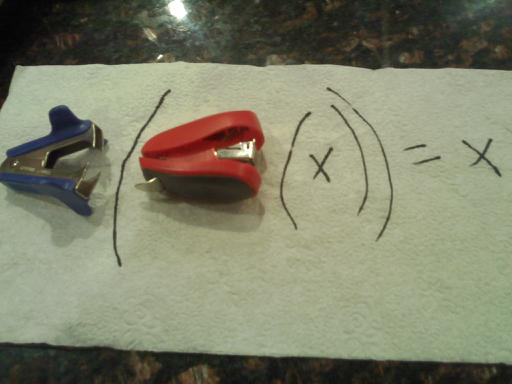
\includegraphics[scale=.4]{stapler.jpg}
\end{center}

The stapler puts things together with a staple. The staple remover separates things by removing a staple. So they are inverse functions.\\

For one function to be the opposite of the other it must have the opposite \textit{operations}\\

\begin{center}
\begin{tabular}{ c | c }

Function & Inverse \\ \hline

$+$ & $-$\\

$\times$ & $\div$ \\

$x^2$ & $\sqrt{x}$ \\

$x^3$ & $\sqrt[3]{x}$\\

\end{tabular}
\end{center}


If $f(x)$ and $g(x)$ are inverses, then
$$[f \circ g](x)=x$$ $$[g \circ f](x)=x$$\\

English: If two functions are inverses, then when composed the answer is $x$. But to be sure we must compose both ways.\\

\clearpage

\textbf{Example 1:} $d(x)=x+5$ and $b(x)=x-5$. Are they inverses?\\

$[d \circ b](x)=$\\

\vspace{.65in}

$[b \circ d](x)=$\\

\vspace{.65in}

\textbf{Example 2:} $j(x)=2x-1$ and $k(x)=2x+1$. Are they inverses?\\

$[j \circ k](x)=$

\vspace{.65in}

$[k \circ j](x)=$\\

\vspace{.65in}

\textbf{Example 3:} $p(x)=x^2+2$ and $q(x)=\sqrt{x+2}$. Are they inverses?\\

$[p \circ q](x)=$\\

\vspace{.65in}

$[q \circ p](x)=$\\

\vspace{.65in}

\textbf{Example 4:} $f(x)=\frac{x}{2}-4$ and $g(x)=2x+8$\\

$[f \circ g](x)=$\\

\vspace{.65in}

$[g \circ f](x)=$\\



\subsection{Creating Inverse Functions}

We know that when a function is composed into its inverse the result is just $x$. How do we create inverse functions though?\\

\textbf{Step 1:} Change $f(x)$ into a $y$. \\

\textbf{Step 2:} Switch $x$ and $y$.\\

\textbf{Step 3:} Solve for $y$. You should get $y=.....$\\

\textbf{Step 4:} replace $y$ with $f^{-1}(x)$\\

\hrulefill

\textbf{Example 1:} Find the inverse of $f(x)=7x-3$

\begin{enumerate}
\item $y=7x-3$\\

\item $x=7y-3$\\

\item $x+3=7y \longrightarrow y=\frac{x+3}{7}$\\

\item $f^{-1}(x)=\frac{x+3}{7}$
\end{enumerate}

\textbf{Example 2:} Find the  inverse of $p(x)=x^2-9$\\

\vspace{1 in}

\textbf{You Try:} Find the inverse of $h(x)=2x-10$\\

\clearpage

\subsection*{Calculating Inverse Functions}

\hfill NAME:\underline{\hspace{3in}}

\hfill DATE: \underline{\hspace{2in}}


\textbf{Directions:} Determine if the functions are inverses.\\

\begin{enumerate}
\setlength\itemsep{2cm}

\item $a(x)=2x+1$\\

		$b(x)=\frac{x}{2}-1$\\
		
\item $c(x)=\sqrt{x+10}$\\

		$d(x)=x^2 -10$\\
		
\item $t(x)=8x^2 + 13$\\

		$u(x)=\sqrt{\frac{x-13}{8}}$

\end{enumerate}

\vspace{2cm}

\textbf{Directions:} Create the inverse function of each function given.\\
\begin{enumerate}[resume]
\setlength\itemsep{1.2cm}


\item $f(x)=\random x$\\

\item $g(x)=\random x + \random$\\

\item $h(x)=\frac{x}{\random}$\\

\item $j(x)=\frac{\random}{x}$\\

\item $k(x)=\frac{2x}{\random}+\random$\\

\item $m(x)=\sqrt{\random x}$\\

\item $n(x)=\sqrt{\random x + \random}$\\

\item $p(x)=\sqrt{\random x + \random} +\random$\\

\item $q(x)=x^2+ \random$\\

\item $r(x)=(2x)^2 + \random$\\

\end{enumerate}

\textbf{Challenge Problem:} $f(x)=\frac{3x^2+1}{2}-\random$

\clearpage

\subsection{Graphs of Inverse Functions}

Graphs of inverse functions are always \textit{reflections} over the line $y=x$ (yes, the same $x$ that's a solution when we find they're inverses).\\

Another way of saying this is that if $(a,b)$ is a point 

$$(a,b) \in f(x) \Leftrightarrow (b,a) \in f^{-1}(x)$$

That's another way of saying: switch the $x$ and $y$.\\

\textbf{Example 1)}

\color{red}$$f(x)=5x-4$$
\color{blue}$$f^{-1}(x)=\frac{x+4}{5}$$ \color{black}

\begin{center} 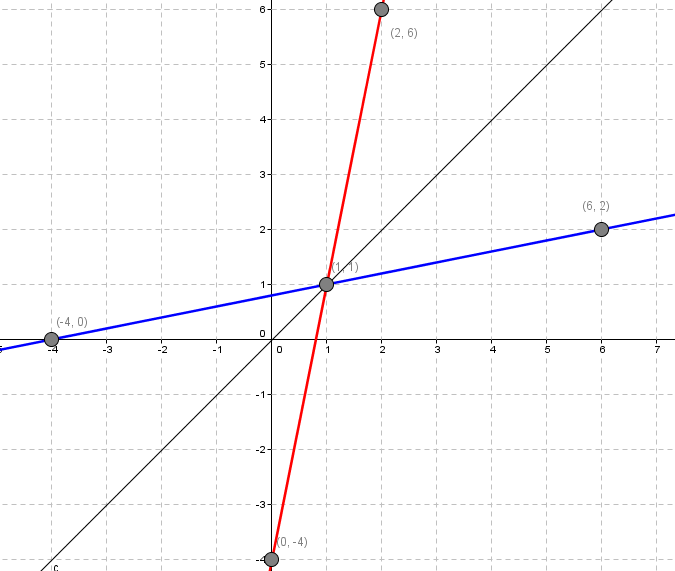
\includegraphics[scale=.5]{inverse1.png} \end{center}

\begin{multicols}{2}
	\begin{center}
	\color{red}
	\begin{tabular}{c | c}
	
		\hspace{.5cm}$x$\hspace{.5cm} & $y$ (or $f(x)$) \\ \hline

		0 & -4 \\
		1 & 1 \\
		2 & 6
	
	\end{tabular}


	\color{blue}
	\begin{tabular}{ c | c }
		\hspace{.5cm} $x$\hspace{.5cm} & $y$ (or $f^{-1}(x)$) \\ \hline
		-4 & 0\\
		1 & 1\\
		6 & 2 \\
	\color{black}
	\end{tabular}
\end{center}
\end{multicols}

The values of the points are reversed. There is also a reflection over the line $y=x$ \\ 

Geogebra demo. Download Geogebra!



\textbf{Example 2)} No graph necessary

\color{red} $$g(x)=2x-1$$
\color{blue} $$g^{-1}(x)=\frac{x+1}{2}$$ \color{black}

\begin{multicols}{2}
\begin{center}
	\begin{tabular}{c | c}
	
		\hspace{.5cm}$x$ \hspace{.5cm}& $y$ (or $g(x)$) \\ \hline
	
		-2 & -5\\
		
		-1 & -3\\
		
		0 & -1 \\
		
		1 & 1 \\
		
		2 & 3 \\
	
	\end{tabular}
	
		\begin{tabular}{c | c}
	
		\hspace{.5cm}$x$\hspace{.5cm} & $y$ (or $g^{-1}(x)$) \\ \hline
		
		-5 & \\
		
		-3 & \\
		
		-1 &  \\
		
		1 & \\
		
		3 & \\
	
	\end{tabular}

\end{center}
\end{multicols}

\hrulefill

\textbf{You Try:} Fill in the t-chart with the values of the inverse function based on the information of the regular function.\\

 $$p(x)=3x+4$$
 $$p^{-1}(x)=\frac{x-4}{3}$$\\

\begin{multicols}{2}
\begin{center}
	\begin{tabular}{c | c}
	
		\hspace{.5cm}$x$ \hspace{.5cm} & $y$ (or $g(x)$) \\ \hline
	
		-2 & -2\\
		 
		-1 & 1\\
		
		0 & 4 \\
		
		1 & 5 \\
		
		2 & 8 \\
	
	\end{tabular}
	
		\begin{tabular}{c | c}
	
		\hspace{.5cm}$x$\hspace{.5cm} & $y$ (or $g^{-1}(x)$) \\ \hline
		 & \\
		 & \\
		 & \\
		 & \\
		 & \\
		
		
	\end{tabular}

\end{center}
\end{multicols}
 
 

\section{Review}

Mr. Wolf \hfill NAME:\underline{\hspace{3in}}\\ 
Pre-Calc \\ 
$MC^2$ High School \hfill DATE:\underline{\hspace{2in}}\\
2014-2015\\

\textbf{Operations with Function Notation}\\

$$a(x)=4x-13 \hspace{.3in} b(x)=9x \hspace{.3in} c(x)=x^2$$\\

Complete the following operations on the functions (2 points each)\\

\begin{enumerate}
\begin{multicols}{2}
	\setlength\itemsep{1cm}

	\item $[a+b](x)=$\\
	
	\item $[a+c](x)=$\\
	
	\item $[b-a](x)=$\\
	
	\item $[b \cdot c](x)=$\\
	
	\item $c(5)=$\\
	
	\item $c(-5)=$\\
	
	\item $a(3h-2)=$\\

\end{multicols}
\end{enumerate}

\hrulefill

$$k(x)=7x+7 \hspace{1in} h(x)=\frac{x}{7}-1$$

\begin{enumerate}[resume]
	\setlength\itemsep{1cm}
	
	\item $[k\circ h](x)=$\\
	
	\item $[h \circ k](x)=$\\
	
	\item are $h$ and $k$ inverses?\\
	
	\item Write the inverse of $p(x)=2x-1$\\
	
		\vspace{1in}
		
	\item Fill out the t-chart for $p(x)$
	
	\begin{center}
	\begin{tabular}{c | c}
	
		\hspace{.5cm}$x$ \hspace{.5cm} & $y$ (or $p(x)$) \\ \hline
	
		-2 & \\
		 
		-1 & \\
		
		0 &  \\
		
		1 &  \\
		
		2 &  \\
	
	\end{tabular}
	\end{center}
	
	\item List the domain and range of the t-chart\\
	
	\item Fill the t-chart for $p^{-1}(x)$\\
		\begin{center}
		\begin{tabular}{c | c}
	
		\hspace{.5cm}$x$ \hspace{.5cm} & $y$ (or $p(x)$) \\ \hline
	
		& \\
		 
		& \\
		
		&  \\
		
		&  \\
		
		&  \\
	
	\end{tabular}
	\end{center}	
\end{enumerate}



\section*{Quiz Review 2}

Mr. Wolf \hfill NAME:\underline{\hspace{3in}}\\ 


\textbf{Operations with Function Notation}\\

$$a(x)=3x-10 \hspace{.3in} b(x)=2x \hspace{.3in} c(x)=x^2$$\\

Complete the following operations on the functions (2 points each)\\

\begin{enumerate}
\begin{multicols}{2}
	\setlength\itemsep{1cm}

	\item $[a+b](x)=$\\
	
	\item $[a+c](x)=$\\
	
	\item $[b-a](x)=$\\
	
	\item $[b \cdot c](x)=$\\
	
	\item $c(10)=$\\
	
	\item $c(-7)=$\\
	
	\item $a(2k+15)=$\\

\end{multicols}
\end{enumerate}

\hrulefill

$$k(x)=\frac{x}{2}-3 \hspace{1in} h(x)=2x+6$$

\begin{enumerate}[resume]
	\setlength\itemsep{1cm}
	
	\item $[k\circ h](x)=$\\
	
	\item $[h \circ k](x)=$\\
	
	\item are $h$ and $k$ inverses?\\
	
	\item Write the inverse of $p(x)=5x-10$\\
	
		\vspace{1in}
		
	\item Fill out the t-chart for $p(x)$
	
	\begin{center}
	\begin{tabular}{c | c}
	
		\hspace{.5cm}$x$ \hspace{.5cm} & $y$ (or $p(x)$) \\ \hline
	
		-2 & \\
		 
		-1 & \\
		
		0 &  \\
		
		1 &  \\
		
		2 &  \\
	
	\end{tabular}
	\end{center}
	
	\item List the domain and range of the t-chart\\
	
	\item Fill the t-chart for $p^{-1}(x)$ (from answer to 11)\\
		\begin{center}
		\begin{tabular}{c | c}
	
		\hspace{.5cm}$x$ \hspace{.5cm} & $y$ (or $p^{-1}(x)$) \\ \hline
	
		& \\
		 
		& \\
		
		&  \\
		
		&  \\
		
		&  \\
	
	\end{tabular}
	\end{center}	
\end{enumerate}



\section*{Quiz}

Mr. Wolf \hfill NAME:\underline{\hspace{3in}}\\ 
Pre-Calc \\ 
CMSD-JFK \hfill DATE:\underline{\hspace{2in}}\\
2014-2015\\

\textbf{Operations with Function Notation}\\

$$a(x)=3x-10 \hspace{.3in} b(x)=5x \hspace{.3in} c(x)=x^2$$\\

Complete the following operations on the functions (2 points each)\\

\begin{enumerate}
\begin{multicols}{2}
	\setlength\itemsep{1cm}

	\item $[a+b](x)=$\\
	
	\item $[a+c](x)=$\\
	
	\item $[b-a](x)=$\\
	
	\item $[b \cdot c](x)=$\\
	
	\item $c(2)=$\\
	
	\item $b(-3)=$\\
	
	\item $a(7r)=$\\

\end{multicols}
\end{enumerate}

\hrulefill

$$k(x)=2x+6 \hspace{1in} h(x)=2x-6$$

\begin{enumerate}[resume]
	\setlength\itemsep{1cm}
	
	\item $[k\circ h](x)=$\\
	
	\item $[h \circ k](x)=$\\
	
	\item are $h$ and $k$ inverses?\\
	
	
	\item Calculate the inverse of $p(x)=3x+2$\\
	
		\vspace{1in}
		
	\item Fill out the t-chart for $p(x)$
	
	\begin{center}
	\begin{tabular}{c | c}
	
		\hspace{.5cm}$x$ \hspace{.5cm} & $y$ (or $p(x)$) \\ \hline
	
		-2 & \\
		 
		-1 & \\
		
		0 &  \\
		
		1 &  \\
		
		2 &  \\
	
	\end{tabular}
	\end{center}
	
	\item List the domain and range of the t-chart\\
	
	\item Fill the t-chart for $p^{-1}(x)$\\
		\begin{center}
		\begin{tabular}{c | c}
	
		\hspace{.5cm}$x$ \hspace{.5cm} & $y$ (or $p(x)$) \\ \hline
	
		& \\
		 
		& \\
		
		&  \\
		
		&  \\
		
		&  \\
	
	\end{tabular}
	\end{center}	
\end{enumerate}

\vspace{.5in}

\textbf{Extra Credit:} What is the answer to the extra credit question?

\pagebreak

\begin{enumerate}
\item $(x^2+5x-3)+(4x^2-9x+12)$\\

\item $(xy^3+2x-7y+3)-(x^2+2xy^3+2x-y+10)$\\

\item $(2x-1)(3y+3)$\\

\item $(3x-2)^2$\\
\end{enumerate}

\end{document}
